
\part{Hybridity}
\section{Why Hybrid}

Virtually all optical phenomena can be modelled using ray tracing. The same can not be said for rasterization. 

\subsection{Rendering effects that are tricky using rasterization}

	\paragraph A typical problem with rasterization is the blending order of fragments needed for translucent surfaces. This is required if a scene contains more than one planar glass surface or any curved glass. Blending order can be solved using an A-buffer \cite{carpenter_1984} at the cost of program complexity and memory. 

	\paragraph Shadows using shadow maps have many problems. Ray tracing dosn't suffer aliasing to the same extent.

	\paragraph Reflections must be done by rendering the scene seen from the surface that is to recieve reflections. Usually the scene is rendered into a cube map using six cameras. This is a crude approximation. Creating multiple reflection bounces quickly becomes more expensive. All surfaces visible in the reflection must be rendered multiple times. A ray tracer in comparison only needs traverse the rays affected.

	So, will we in the future, once computational power is good enough to raytrace at retinal display quality only use ray tracing? Probably not. We surround ourselves with objects that essentially only have diffuse shading. Glass house and porcelain shops are the exception, and even in such scenes, there are an abundance of diffuse surfaces.

	Raytracing is essential for reflections. Just look at this car:

	\begin{figure}[ht]
		\centering
		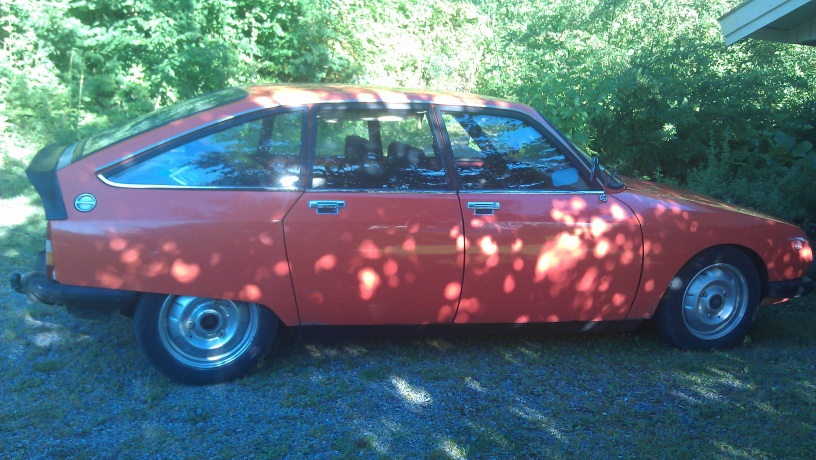
\includegraphics[width=0.80\textwidth]{Media/why_hybrid_carphoto.jpg}
		\caption{The car paint, glass and chrome details are essentially the only reflective surfaces in the scene}
		\label{fig:citroen_gs}
	\end{figure}
	
	\paragraph{Fill(rate) workload}
	With rasterization, we often tell the GPU to shade large surfaces that's out of view, the GPU quickly clips and discards fragments out side the view frustum. Pixar, as mentioned earlier solves this by cutting the geometry until it fits.

	Ray tracing doesn't have this problem. We only try to shade what is visible.

	\paragraph For a raster to be able to render anything, it must be converted to triangles. There are types of geometry where it may be more efficient in both terms of speed and memory to use a raytracer.

	Some examples are:
	\begin{itemize}
		\item Distance Fields can be raymarched, or an iso value can be extracted by solving the fields equation in an analytic raytracer. A rasterizer must usually sample all of the         field inside the view volume. This becomes especially problematic if the field changes on a frame-by-frame basis.

		\item Scalar Volume Data. Instead of rendering slices or iso-surfaces, the raw data can be sampled using discrete raytracing (also known as ray marching). %cite [Kajiya1986] The rendering equation ???

		\item Spline surfaces
		\item Perfect analytical surfaces
	\end{itemize}

\subsection{Reasons to use a hybrid}

Its the future. Hardware is becoming increasingly parallel. Ray tracing is trivially parallellizable. Ray tracing won't replace rasterization over night, but it will become increasingly useful.

Its conceptually simpler. Shaders can be written with fewer dependencies. Trading memory and programmer time for compute power.

As mentioned, certain types of geometry are better suited for ray tracing.

Rasterization has recieved a lot of attention due to its efficiency. This efficiency is mainly due to its cache and bandwidth friendliness. Unless someone invents memory with bandwidth on par with CPU Registers, ray tracing will allways be slower.

	\begin{figure}[ht]
		\centering 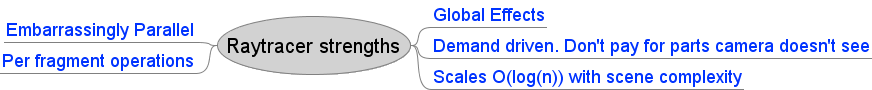
\includegraphics[width=0.80\textwidth]{Media/why_hybrid_raymindmap.png}
		\caption{ray tracer strengths}
		\label{fig:ray_mmap}
	\end{figure}
	
	\begin{figure}[ht]
		\centering 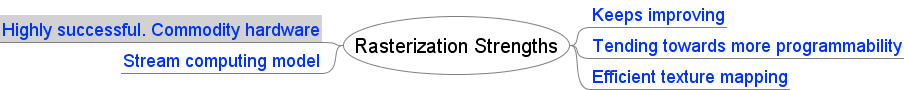
\includegraphics[width=0.80\textwidth]{Media/why_hybrid_rastermindmap.png}
		\caption{raster strengths}
		\label{fig:raster_mmap}
	\end{figure}

In a raytracer, global effects \ref{fig:ray_mmap}, such as reflections, refractions and shadows, are handled per fragment.

\ref{fig:citroen_gs}